%
% First comes an example EPS file -- just ignore it and
% proceed on the \documentclass line
% your LaTeX will extract the file if required
\begin{filecontents*}{example.eps}
%!PS-Adobe-3.0 EPSF-3.0
%%BoundingBox: 19 19 221 221
%%CreationDate: Mon Sep 29 1997
%%Creator: programmed by hand (JK)
%%EndComments
gsave
newpath
  20 20 moveto
  20 220 lineto
  220 220 lineto
  220 20 lineto
closepath
2 setlinewidth
gsave
  .4 setgray fill
grestore
stroke
grestore
\end{filecontents*}
%
\RequirePackage{fix-cm}
%
\documentclass{svjour3}                     % onecolumn (standard format)
%\documentclass[smallcondensed]{svjour3}     % onecolumn (ditto)
% \documentclass[smallextended]{svjour3}       % onecolumn (second format)
%\documentclass[twocolumn]{svjour3}          % twocolumn
%
\smartqed  % flush right qed marks, e.g. at end of proof
%
\usepackage{graphicx}
\usepackage[most]{tcolorbox}
\usepackage{listings}
\usepackage{xcolor}

\lstset{
    language=Python,
    basicstyle=\ttfamily,
    keywordstyle=\color{blue},
    stringstyle=\color{red},
    commentstyle=\color{green},
    morecomment=[l][\color{magenta}]{\#}
}

%
% \usepackage{mathptmx}      % use Times fonts if available on your TeX system
%
% insert here the call for the packages your document requires
%\usepackage{latexsym}
% etc.
%
% please place your own definitions here and don't use \def but
% \newcommand{}{}
%
% Insert the name of "your journal" with
% \journalname{myjournal}
%
\begin{document}

\title{Exploring the Role of Feedback in Machine Learning Jupyter Notebooks}

%\titlerunning{Short form of title}        % if too long for running head

\author{Arumoy Shome\and
  Lu{\`\i}s Cruz\and
  Diomidis Spinellis\and
  Arie van Deursen
}

%\authorrunning{Short form of author list} % if too long for running head

\institute{A. Shome \at
  Delft University of Technology\\
  \email{a.shome@tudelft.nl}
  \and
  L. Cruz \at
  Delft University of Technology\\
  \email{l.cruz@tudelft.nl}
  \and
  D. Spinellis \at
  Delft University of Technology\\
  \email{d.spinellis@tudelft.nl}
  \and
  A. V. Deursen \at
  Delft University of Technology\\
  \email{arie.vandeursen@tudelft.nl}
}

\date{Received: date / Accepted: date}
% The correct dates will be entered by the editor


\maketitle

\begin{abstract}
Insert your abstract here. Include keywords, PACS and mathematical
subject classification numbers as needed.
\keywords{First keyword \and Second keyword \and More}
% \PACS{PACS code1 \and PACS code2 \and more}
% \subclass{MSC code1 \and MSC code2 \and more}
\end{abstract}

\section{Introduction}

\section{Methodology}
% For one-column wide figures use

\begin{figure}
  \centering
  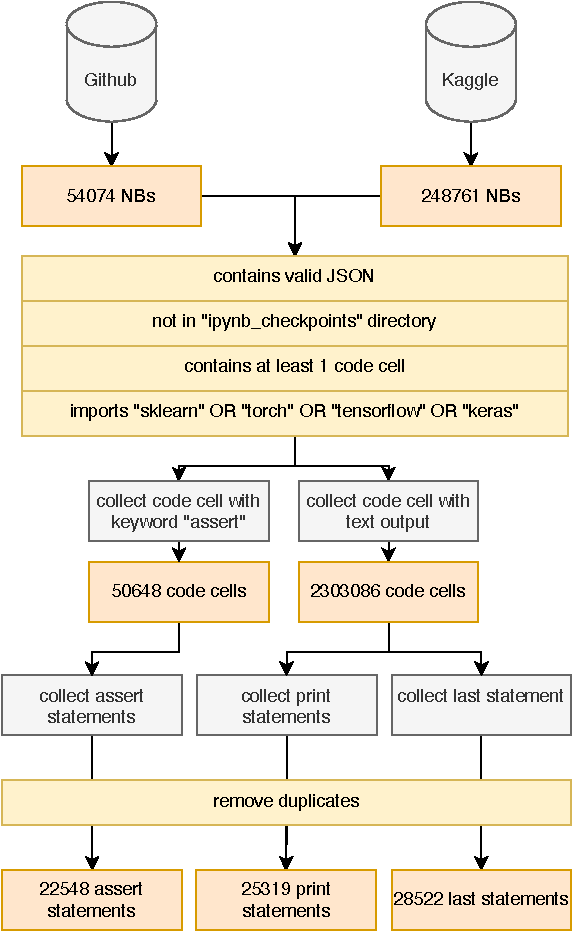
\includegraphics[width=\linewidth]{esem24-method.pdf}
  \label{fig:data-collection}
  \caption{Overview of data collection methodology used in this study}
\end{figure}

\section{Results}

% TODO: for each of the feedback types; start with the descriptive and lexical analysis we performed
% TODO: then move into the case studies, and link them to existing literature; use the fault and failure taxonomies; perhaps also link the feedbacks to ML lifecylce proposed by Amershi 2019?

\subsection{Implicit feedback using \texttt{print} statements and output of code cells}

\subsubsection{Data distribution check (O2, O4, O9, O14, O20, O25, O48)}
% a mix of visualisations and pandas dataframes that show the distribution of a column in the data
% we primarily observe these checks being used to determine the relationship of a feature with the target feature
% typically in the EDA/data exploration/understanding phase
% several examples where the distribution of a newly created feature is checked (binning a continuous feature into categorical one)
% one uses descriptive statistics to verify that data normalisation worked (again, a check after data transformation step)

We observe the use of visualisations and dataframes to check the distribution of a feature. Often, the analysis is performed in the context of a multivariate analysis, where the distribution of a feature is checked against all possible outcomes of the target feature.

Typically, this check is performed in the EDA phase where the author is trying to understand the relationship of a feature with the target feature. This done to identify features that can be used to train the ML model.

We also observe that the distribution of a feature is checked directly after creating it. For example, we observe this check after converting a continuous feature into a categorical feature using binning. Another example is the use of descriptive statistics provided by pandas to check that the prior data normalisation step worked (the author manually verified the mean and standard deviation of the feature from the output).

\subsubsection{Data relationship check (O6, O10)}

Linear regression models assume a linear relationship between the features in the training data, with the target feature. We see this being verified using lineplots to check the presence of a linear trend between a given feature and the target feature.

A special case is O10 which uses a regplot. This is a visualisation provided by the seaborn library that plots the data along with a linear regression model fit.

\subsubsection{Dependency check (P71, P86)}

We find evidence of lack of software engineering best practise. Dependencies should be manage with external programs built for this task. Python has a built-in functionality for this, where dependencies along with version can be specified in a requirements.txt file. There are also several external programs such as the use of lockfiles by pipenv and poetry which lock a specific version of a dependency such that all files are reproducible on all systems.

P71 prints the version of an external library which the author is expected to verify manually. P86 prints a confirmation message if the Cuda library is available on the system where the notebook is being executed.

\subsubsection{Execution time check (P66)}

Often several ML models are trained and for a single task. The selection is based on requirements that not only consider the performance of the model, but also the total time required to train the model. Since this is an iterative task, a model that can be more efficiently retrained, helps reduce costs in the long run, and has been proven to be more sustainable.

P66 is from a notebook where several models are trained for the same task, and their performance along with the time taken to train is printed. The cells of a notebook are also executed several times, for a long running cell (such as the ones that train the model), an indication of the total execution time helps (after the first run, the author has a baseline for the time it will take).

\subsubsection{Missing value check (O12, O36, P74)}

Check if missing values are present in any features of the data. After loading the dataset and in the EDA phase of analysis.

From our data smells paper: descriptive statistics functions typically ignore missing values; leading to biased and incorrect results and conclusions

ML models also except numerical values, a null type value raises an exception (since computations cannot be performed)

P74 and O36 is an aggregated check over the entire dataset.

% TODO: highlight the use of visualisations to check for missing values; what is the benefit of using a visualisation instead of code?
More interesting is O12 which uses a heatmap to show the distribution of the missing values across all features of the dataset.

\subsubsection{Model performance check (O3, O50, O52, O57, O74, P3, P6, P8--12, P16--19, P23, P24, P28, P30, P34, P42, P47, P48, P50, P51, P54, P55, P57, P58, P61, P78, P93)}

The performance is printed to compare against other models/variations in the experimental model development phase; during the continuous experimentation phase, the author might change parameters of the model or change the data (engineer features, etc) and then re-run the model to check if the performance improved

Mean accuracy over K-fold validation

Other performance metrics such as recall, precision and F1 also printed

Error in predictions (RMSE, MSE)

P48: prints the loss

% TODO: whats the point of this?
P54: print the intercept of linear regression model

Classification report is used to produce a summary of popular performance metrics such as accuracy, recall, precision and F1.

Precision and recall is checked using the confusion matrix.

% TODO: highlight the need for normalising vs. comparing absolute values; the data might be imbalanced so does not make sense to compare the absolute values
O3: use heatmap to visualise the confusion matrix of a multi-label classification task. The values are normalised using the actual number of examples of each class which makes the comparisons of the values across the classes possible.

O52: author wrote a custom function which gets the predictions of an image classifier (developed in the NB) on a random sample of images. The predictions along with the input image is printed. The author is manually spot-checking the accuracy of the predictions. Or perhaps trying to find examples that produce the wrong prediction?

\subsubsection{Model architecture (P92)}

Several neural network architectures are available as part of the ML library (for instance keras, pytorch and tensorflow come pre-loaded with several NNs).

Print the architecture of the neural network. The layers of the model, neurons in each layer and the activation functions are printed in a text diagram.

\subsubsection{Resource check (O64, O66, P68, P82, P107)}

Check is GPU or TPU resources are available. We suspect these checks are coming from Google Colab notebooks where computation can be off-loaded to remote hardware.

In P107, check that the pre-trained model was successfully loaded from the file system.

\subsubsection{Shape check (P4, P32, P117)}

% TODO: why is shape check important?
Checking the shape of the data is important for several reasons. If we perform some data pre-processing or transformation, we want to ensure that the shape of the data is the same as expected.

Number of features in the training and testing data must match. When using statistical ML models, the model "fits" the training data and thus expects the same shape in the testing data to make inference. When developing neural networks, architectural decisions such as the number of input neurons is made based on the shape of the data.

During the testing shape, the number of examples in the test input must be the same as the number of labels so that the performance metrics such as accuracy, can be correctly calculated.

\subsubsection{Type check (O71, P43)}

All ML models expect the input data to be entirely numerical, so that mathematical operations such as matrix multiplications may be carried out without errors.

Checking the data type in the EDA phase may be done to understand the optimal data pre-processing or transformation techniques necessary, to make the data ready for model. For instance, numerical features may need to be normalised while categorical features need to one-hot encoded.

\subsubsection{Value check/ Spot checks (O56, O60, P64, P67, P114)}
% NOTE: perhaps these are spot-checks?

O56: check the prediction of the model on a single input image

O60: check the number of features in the data is equal to the expected number after performing PCA, the author checks the head of the dataframe and manually verifies the number of features

P64: find the max in the second channel of a 3D numpy array (highlight this case study; this is done for image processing!)

P67: manually verify the output of an activation function in a neural network against expected value.

P114: check that one-hot encoding worked

\subsubsection{Model training (O8, O31, O42, P77)}

O8, P77: Periodically print the progress made in training by printing the training loss/accuracy of model.

O31: check the model fits the data without any errors; this is done in the model experimentation phase, where several models are tested and the best one based on the selection criteria is picked

\subsection{Explicit feedback using \texttt{assert} statements}

% TODO: find out more about batch training
\subsubsection{Batch size check (A21, A28, A70)}

Neural Networks are trained using smaller batches that makes it more efficient use of hardware GPU cores. During batch training the weights are not updated with every example but with the average of the entire batch, this ensures a more optimal and smoother learning curve and generally leads to better generalizability.

When trained using batches, we need to take this into account when calculating the performance of the model. We need to calculate the accuracy over multiple batches and then average the results.

We encounter assertions that check the size of the batch prior to training. This is to ensure that the batch size matches the hardware specifications? We should not have a batch size that does not fit in the memory of GPU/CPU.


\subsubsection{Data leakage check (A33)}

It is a best practise to ensure that the ML model is not tested using examples that it has already encountered during training. This is to ensure that the model is not overfitting on the training data and is able to generalise to examples similar to the distribution of the training set, but not exactly the same. In A33 we see that the assert ensures that the training and validation sets do not share any examples.

\subsubsection{Dependency check (A18, A67)}
% TODO: what is the motivation of this assertion? Find prior work on python dependency management?

This is a unique type of test which occurs due to the unique workflow of notebooks. Typically dependencies are managed through external means such as dedicated dependency management solutions or the builtin Python method using a requirements.txt file. We notice assertions that check that the major version of an external dependency is equal to the specified value.

% NOTE: missing-value-check and existence-check

\subsubsection{Existence check (A86)}

Existence checks are carried out in various contexts. Most are for checking that columns in a dataset do not contain missing values. Others ensure that certain columns (such as the column containing the labels of the data) exists in the dataset prior to splitting the data into training and testing sets. Existence checks are frequently performed after data pro-processing  steps are performed to ensure that missing values were not added to the dataset.

% TODO: we need to elaborate this one with examples 

\subsubsection{Mathematical property checks (A3, A25, A56, A64)}

Machine learning models are often rooted in statistical models. Implementing neural networks requires a grasp of linear algebra and matrix multiplication. We find several assertions that test the mathematical properties of arrays and matrices after performing matrix operations.

\subsubsection{Model performance check (A7, A15, A19, A22, A24, A26, A38, A54, A58, A59, A72)}

We see several assertions that test for the performance of the trained ML model against a validation or test test. The assertions often compare a performance metric (such as accuracy, precision, recall, F1, etc) against a predefined threshold.

% TODO: this needs more work and investigation
\subsubsection{Network architecture check (A11)}

We only have one example here.

% TODO lots to elaborate and discuss here
\subsubsection{Resource check (A10, A14, A37, A60, A74)}

We find assertions that check that a pre-trained model exists on the file system, or that data can be loaded from a specified file path. There are also checks that ensure that a visualisation created using matplotlib contains data in it.

\subsubsection{Data shape check (A5, A9, A13, A16, A17, A29, A31, A61, A71, A76--78, A82, A84, A85, A89, A90, A91, A93--96, A98--101)}

``Swiss army knife'' of assertions!

\subsubsection{Type check (A2, A35, A40, A81, A88)}

Checking the data type of features and such.

\subsubsection{Value check (A30, A41, A44--46, A52, A65, A68, A69, A73, A92)}

Check that the values in a column are in the specified values (categorical) or in a specified range (normalised continuous variable) or binary (such as the label column).

% NOTE: blanks and unit-tests
\subsubsection{Miscellaneous checks (A6, A20, A32, A34, A36, A53, A62, A75, A83, A87, A97)}

These feel like unit tests, performed in lieu of writing full test suites in the notebook.

\bibliographystyle{ACM-Reference-Format} \bibliography{bibliography}
%\begin{acknowledgements}
%If you'd like to thank anyone, place your comments here
%and remove the percent signs.
%\end{acknowledgements}


% Authors must disclose all relationships or interests that 
% could have direct or potential influence or impart bias on 
% the work: 
%
% \section*{Conflict of interest}
%
% The authors declare that they have no conflict of interest.


% BibTeX users please use one of
\bibliographystyle{spbasic}      % basic style, author-year citations
%\bibliographystyle{spmpsci}      % mathematics and physical sciences
%\bibliographystyle{spphys}       % APS-like style for physics
\bibliography{bibliography}   % name your BibTeX data base

\end{document}
% end of file template.tex

